\chapter{Einleitung}
\section{Pepperl + Fuchs / HMI}
Die \ac{p+f} wurde 1945 von Walter Pepperl und Ludwig Fuchs gegründet. Anfangs war sie eine Radioreperaturwekstadt, welche sich erst nach der Entwicklung eines eigenen Näherungsschalters so wie eines eigensicheren Transistorverstärkers auf das gebiet der Elektronik ausweitete. Inzwischen entwickelt, produziert und vertreibt \ac{p+f} Baugruppen und Sensoren für den Automatisierungsmarkt.\\
\begin{flushleft}
    \begin{figure}[h!]
        \centering
        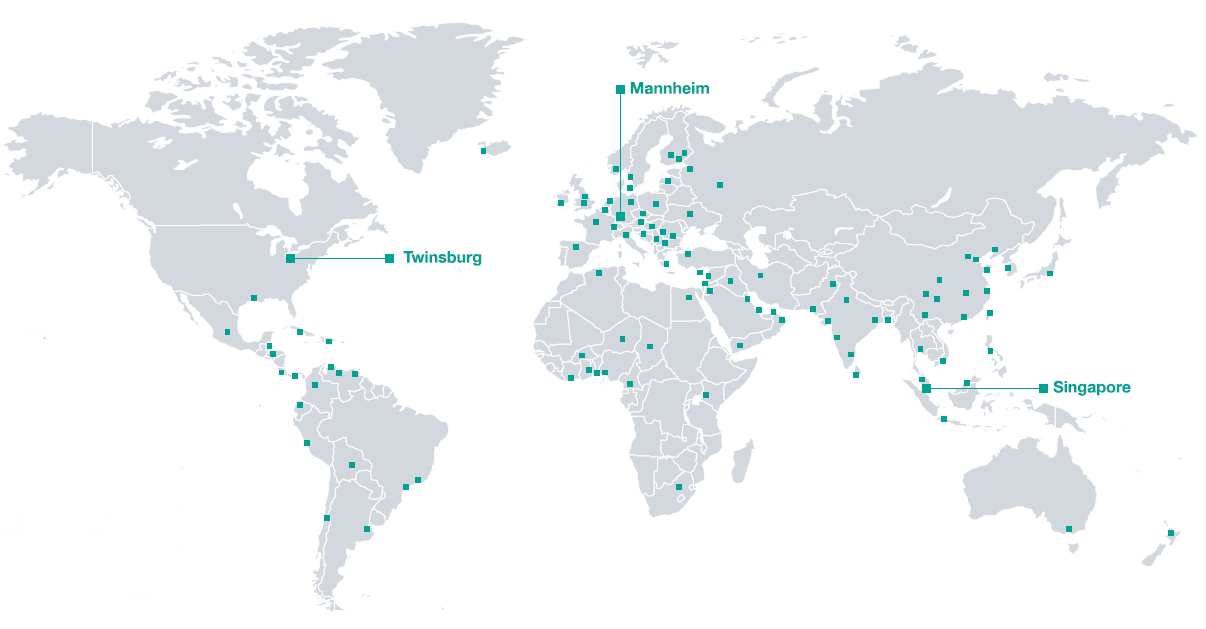
\includegraphics[scale = 0.35]{P+F_Standorte.png}
        \caption{Standorte der Pepperl+Fuchs SE}
        \label{fig:StandortePF}
    \end{figure}
\end{flushleft}
Pepperl\todo{mehr auf HMI eingehen, warum braucht man diese, wo werden die eingesetzt}
Im Bereich der Prozessautomation ist \ac*{p+f} führender Hersteller industrieller Sicherheitsausstattungen. Das Produktportfolio umfasst Trennbarrieren, Signaltrenner, Zener-Barrieren, Feldbus-Technologien, Remote-I/O, HART-Interface-Lösungen, Mensch-Maschine-Schnittstellen (HMI) für Gefahrenbereiche, Füllstandsüberwachung, Überdruckkapselungssysteme, Schaltschränke,Feldverteiler und Warnsysteme für Ex-Umgebungen.\\
Die Abteilung \textit{Human Machine Interfaces} beschäftigt sich dabei mit der Entwicklung von Industrieller Computer Hard- und Software. Dies reicht von zubehör bishin zu vollständige Systemen mit Ex-Umgebungen Zertifizierung. Ziel der Systeme ist die Überwachung und Steuerung sämtlicher Produktionsschritte.   

\section{Problemstellung und Ziel der Arbeit}

\section{Anforderungen}